\documentclass[liststotoc,bibtotoc,fontsize=14pt,]{scrreprt}
\usepackage[utf8]{inputenc} % Zeichenkodierung
\usepackage[ngerman]{babel} % neue deutsche Rechtschreibung
\usepackage{etoolbox}
\setlength{\footskip}{30pt}
\apptocmd{\thebibliography}{\raggedright}{}{}
\usepackage{graphicx}
\usepackage{caption}
\usepackage{subcaption}
\usepackage{url}
\usepackage[onehalfspacing]{setspace}
\usepackage{breakurl}
\usepackage{float}
\usepackage[table,xcdraw]{xcolor}
\usepackage{tabularx}
\usepackage[breaklinks]{hyperref}
\def\UrlBreaks{\do\/\do-}
\usepackage{tocloft}
\usepackage{chngcntr}
\usepackage{listings}
\usepackage{color}
\usepackage[parfill]{parskip}
\definecolor{lightgray}{rgb}{.9,.9,.9}
\definecolor{darkgray}{rgb}{.4,.4,.4} 
\definecolor{purple}{rgb}{0.65, 0.12, 0.82}

\counterwithout{footnote}{chapter}

\deffootnote[2em]{2em}{2em}{%
	\makebox[2em][l]{\bfseries\thefootnotemark}}

\renewcommand{\cftchapdotsep}{\cftdotsep}
\renewcommand{\cftchapleader}{\cftdotfill{\cftchapdotsep}}
\usepackage{amsmath}
\usepackage[paper=a4paper,left=30mm,right=30mm,top=25mm,bottom=25mm]{geometry}
\usepackage[section]{placeins}
\usepackage[font=small,justification=justified]{caption}
\newcommand{\namesigdate}[3][Ort, Datum]{%
	\parbox{\textwidth}{
		\raggedleft #3 
		\vspace{2cm}
		
		\parbox{5cm}{
			\raggedright
			\rule{6cm}{1pt}\\
			#1 
		}
		\hfill
		\parbox{5cm}{
			\raggedright
			\rule{6cm}{1pt}\\
			#2
		}
	}
}


\newcommand*{\tabularwidth}{}
\newdimen\tabularwidth
\usepackage{minitoc}
\hypersetup{
	colorlinks,
	citecolor=black,
	filecolor=black,
	linkcolor=black,
	urlcolor=black
}


\title{Dokumentation Stereo-Fotografie}
\author{Sebastian Degner}

\begin{document}
	%\maketitle
	
	\begin{titlepage}
		\begin{center}
			\vspace{2cm}
			Dokumentation\\ \textbf{Multishot-Technik in der digitalen Fotografie}\\ 
			\vspace{2,5cm}
			
\includegraphics[width=5cm]{HTWK_Logo_RGB-transparent_250.png}\\
			
			\vspace{2,5cm}
			\huge \textbf{\textsf{Dokumentation Stereo-Fotografie}} \\
			\vspace{3cm}
			\fontsize{15}{18} \textbf{Hochschule für Technik, Wirtschaft und Kultur
				Leipzig\\ Fakultät Informatik, Mathematik und Naturwissenschaften\\   Masterstudiengang Medieninformatik}\\
			\vspace{3cm}
		\end{center}
		\normalsize{
			\begin{tabular}{ll}
				Eingereicht von: & {Sebastian Degner} \\
				 & {Sebastian Knabe} \\
				Studiengang: & 15 MIM\\
				Eingereicht am: & 03. März 2017 \\
			\end{tabular}\\
		}
		
	\end{titlepage}
	
	\tableofcontents
	\clearpage
	\listoffigures
	\addcontentsline{toc}{chapter}{Abbildungsverzeichnis}

	\chapter{Einleitung}
	\label{ch:einleitung}
	Im Rahmen des \textit{Moduls Multishot-Technik in der digitalen Fotografie} wurde diese Dokumentation zu dem Thema \textit{High Dynamic Range} (auch mit HDR abgekürzt) realisiert. Mit Hilfe der HDR-Fotografie lassen sich Aufnahmen erstellen, die einen besonders hohen Kontrastumfang aufweisen. Fotos, welche mit dieser Technik aufgenommen werden, können Helligkeitsunterschiede detailreich wiedergeben. Außerdem wird vermieden, dass Bildinformation durch Über- beziehungsweise Unterbelichtung verloren gehen. HDR-Aufnahmen können mit  einer handelsüblichen Spiegelreflexkamera nicht direkt aufgenommen werden. Um diese zu erzeugen, muss man mehrere Einzelbilder aufnehmen, welche später mit Hilfe spezieller Software zu einem HDR-Foto zusammengefügt werden.
	
			
	\chapter{Aufnahmen}
	\label{ch:aufnahmen}
	
	\section{Paulinum }
	\label{sec:spinnerei}

	\subsubsection{Aufnahmeort und -idee}

		\begin{figure}[H]
			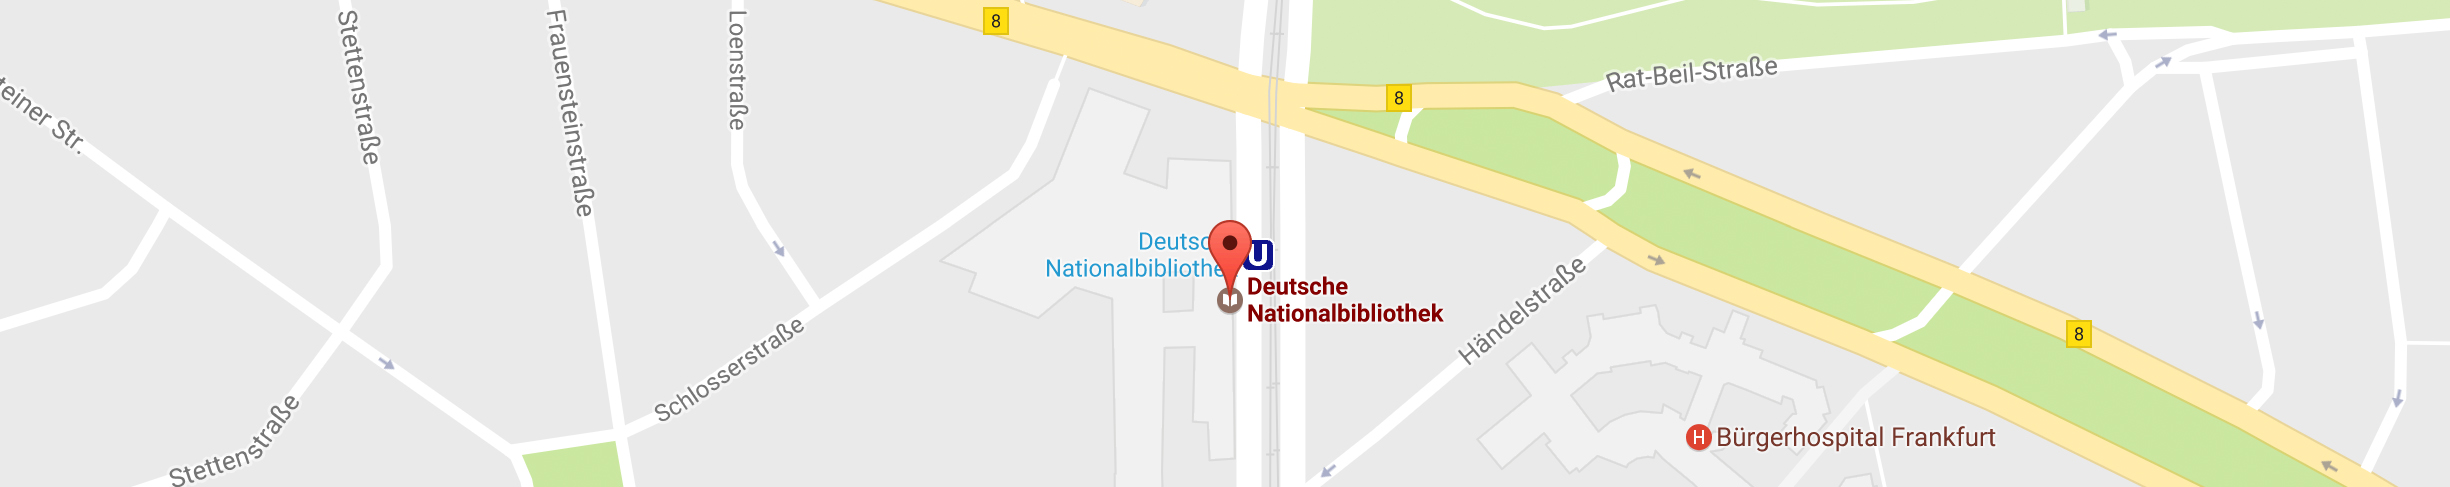
\includegraphics[width=\linewidth]{img/places/bibo_map.jpg}
			\caption{Aufnahmeort Paulinum}
			\label{img:paulinum_map}
		\end{figure}

		\subsubsection{Kameraeinstellungen}
			\begin{minipage}{0.58\textwidth}
				\begin{tabular}{ll}
					Kamera: &Canon EOS 7D \\
					Objektiv: &Canon EF 10-22mm \\
					& F/3.5-4.5 USM\\		
					Brennweite:& 10mm \\
					Belichtungszeit: & $\frac{1}{30}$s /$\frac{1}{15}$s /$\frac{1}{4}$s / $\frac{1}{2}$s \\
					 & 1s\\
					Blendenwert: & f/8\\
					Empfindlichkeit & ISO 100 \\
				\end{tabular}\\
			\end{minipage}%
			\begin{minipage}{0.42\textwidth}
				\begin{figure}[H]
					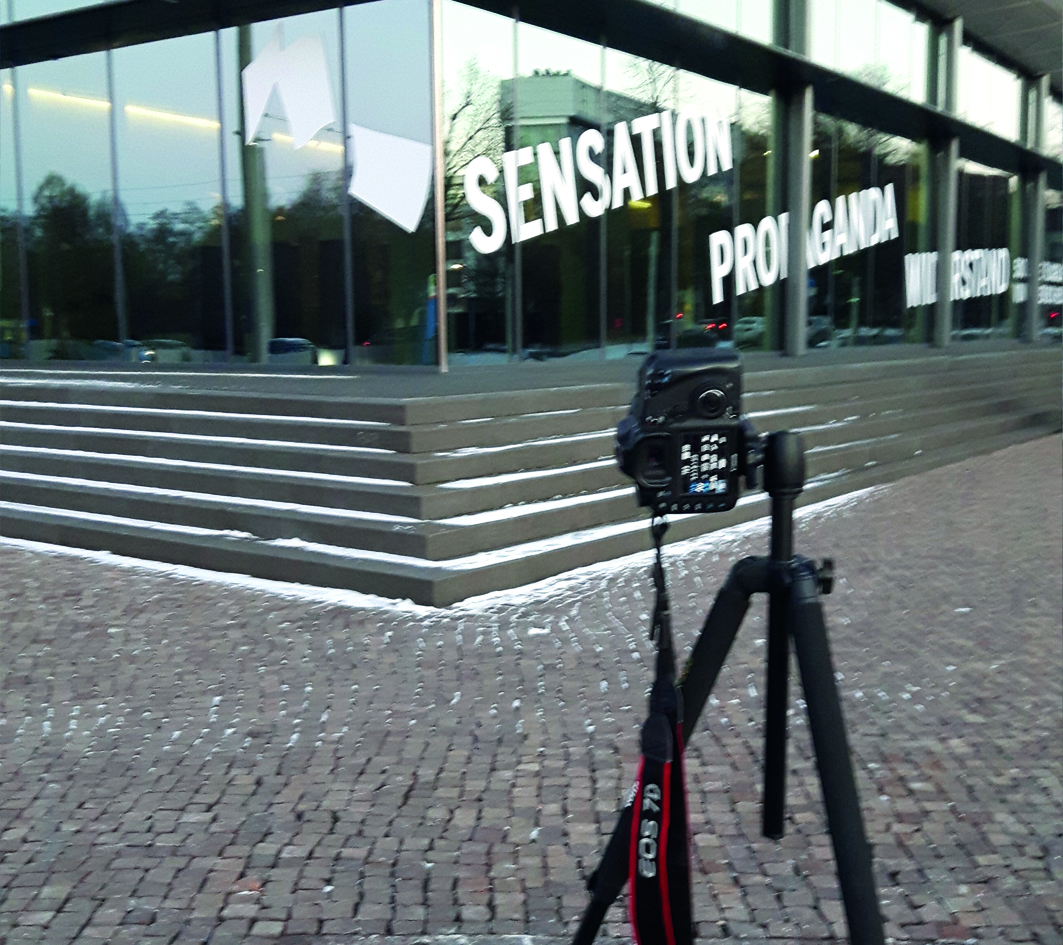
\includegraphics[width=\linewidth]{img/places/bibo.jpg}
					\caption{Aufnahmesituation Paulinum}
					\label{img:ak}
				\end{figure}
			\end{minipage}%

	\subsubsection{Vorgehen}

	
	\newpage
	\begin{figure}[h]
		
\includegraphics[width=\linewidth]{img/ph.jpg}
		\caption{Stereo-Aufnahme Paulinum}
	\end{figure}

\section{Karl-Heine-Denkmal}
\label{sec:palme}
\subsubsection{Aufnahmeort und -idee}



\subsubsection{Vorgehen}

\newpage
\begin{figure}[h]
	
\includegraphics[width=\linewidth]{img/ph.jpg}
	\caption{Stereo-Aufnahme Karl-Heine-Denkmal}
\end{figure}

\section{Leipziger Österreicher-Denkmal}
\label{sec:nikolai}
\subsubsection{Aufnahmeort und -idee}


\subsubsection{Vorgehen}


\newpage
\begin{figure}[h]
	
\includegraphics[width=\linewidth]{img/ph.jpg}
	\caption{Stereo-Aufnahme Österreicher-Denkmal}
\end{figure}
	
	\section{Richard-Wagner-Platz}
	\label{sec:tunnel}
	\subsubsection{Aufnahmeort und -idee}
		
	\subsubsection{Vorgehen}


			 \newpage
			 \begin{figure}[h]
			 	
\includegraphics[width=\linewidth]{img/ph.jpg}
			 	\caption{Stereo-Aufnahme Richard-Wagner-Platz}
			 \end{figure}




	\chapter{Vorbereitung}
		In dieser Arbeit sollen Stereobilder mit unterschiedlichen Kamerasystemen aufgenommen und verglichen werden. Als Spiegelreflexkamera kommt eine Canon 7D mit den Objektiven \textit{Canon EF 10-22mm F/3.5-4.5 USM} und	\textit{Tamron SP 24-70mm F/2.8 Di VC USD} zum Einsatz. Da für eine Stereoaufnahme immer zwei Fotos, um den durchschnittlichen Augenabstand (6,5 cm) versetzt, erstellt werden müssen, ist ein Stereoschlitten notwendig. Dieser besteht im Wesentlichen aus einer Schiene, auf welcher die Kamera verschoben werden kann. Beim Fotografieren wird darauf geachtet, dass eine hohe Schärfentiefe und eine große Tiefenwirkung entsteht.
		
		Die zweite Kamera ist eine Kompaktkamera von Fujifilm und eignet sich im Speziellen für die 3D-Fotografie. Dabei handelt es sich um eine Fujifilm Finepix Real 3D mit zwei Objektiven und entsprechend 2 Sensoren. Sie löst mit 10 Megapixel auf und deckt einen Brennweitenbereich von 35mm bis 105mm ab. Aufgrund dieser Hardware, können beide benötigten Fotosauf einmal geschossen werden. Die Kamera speichert die Einzelaufnahmen als JPG und als Multi Picture Object (MPO) ab. Abgesehen von dieser Funktion, ist die Kompaktkamera einer Spiegelreflexkamera mit guten Objektive stark unterlegen. Besonders störend wirkt sich dabei aus, dass die maximale Dauer einer Langzeitbelichtung nur eine halbe Sekunde beträgt. Soll ein Foto aus einem dunklen Setting normal belichtet sein, muss zwangsweise die ISO angehoben und die Blende geöffnet werden. Auch ist die Menüführung nicht intuitiv, sodass gesuchte Einstellmöglichkeiten umständlich in Untermenüs versteckt sind.
		
		

	\chapter{Nachbearbeitung und Entwicklung}

		\begin{figure}[H]
			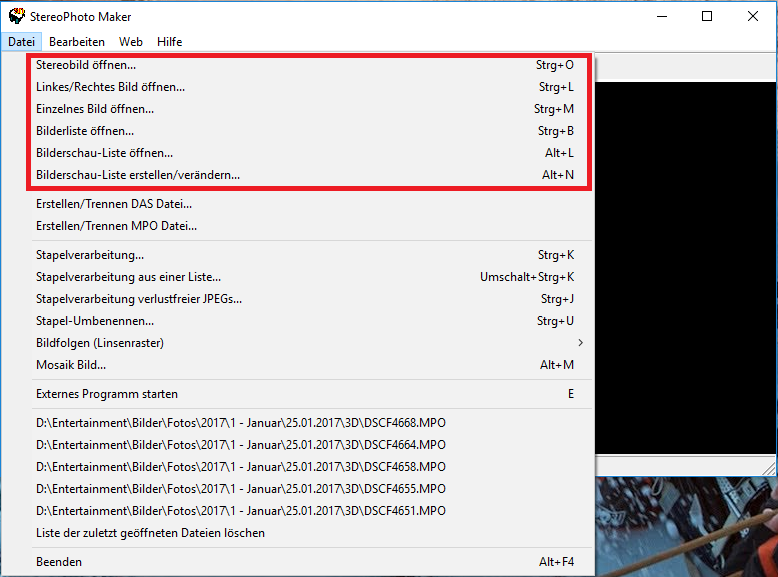
\includegraphics[width=\linewidth]{img/steps/step1.png}
			\caption{StereoPhoto Maker - Import}
			\label{img:maker_import}
		\end{figure}
		
		\begin{figure}[H]
			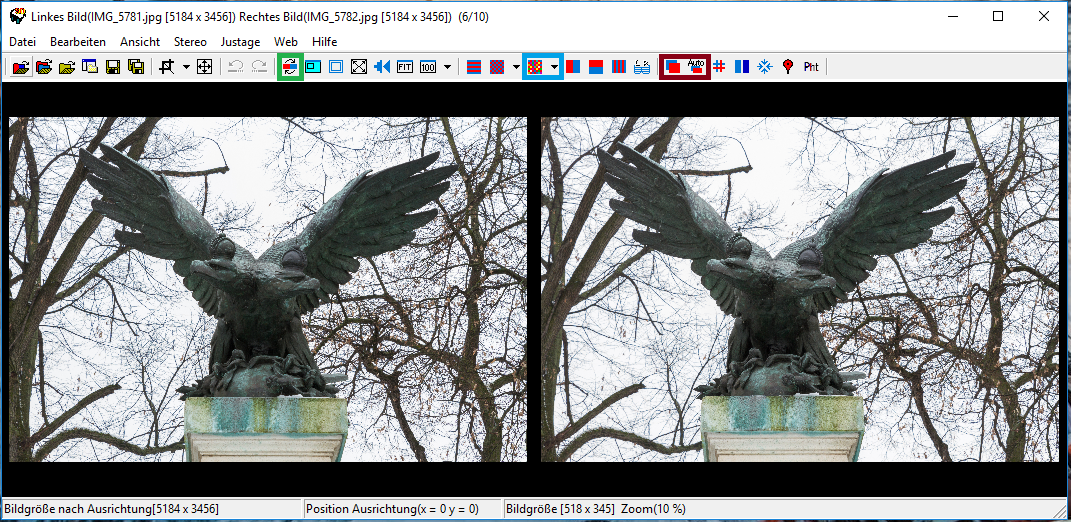
\includegraphics[width=\linewidth]{img/steps/step2.png}
			\caption{StereoPhoto Maker - Darstellung und Optionen}
			\label{img:maker_options}
		\end{figure}
		
		\begin{figure}[H]
			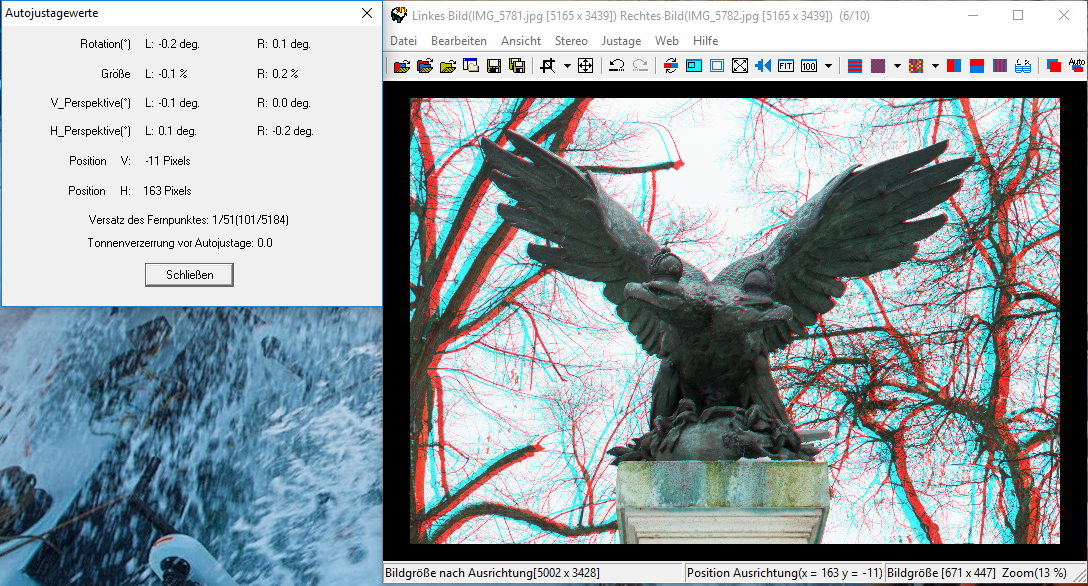
\includegraphics[width=\linewidth]{img/steps/step3.png}
			\caption{StereoPhoto Maker - Autojustage und Zusammenführung}
			\label{img:maker_justage}
		\end{figure}
		
		\begin{figure}[H]
			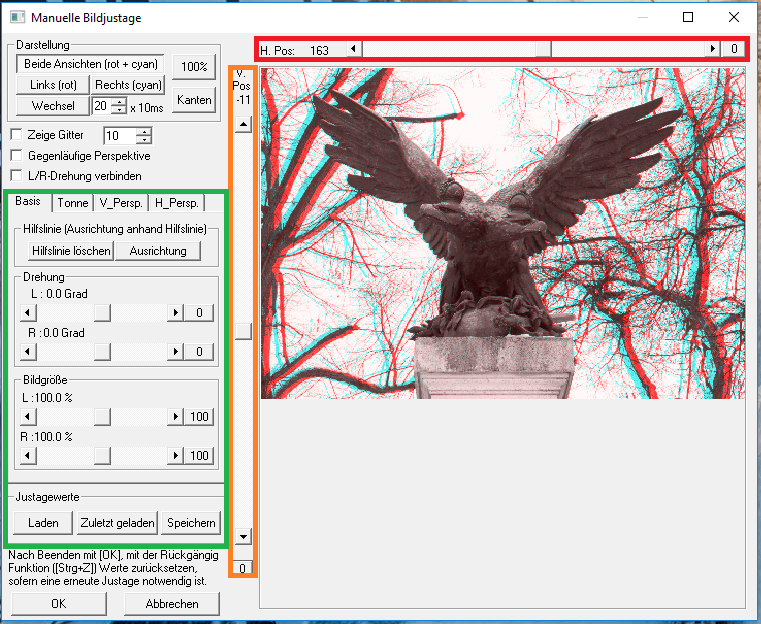
\includegraphics[width=\linewidth]{img/steps/step4.png}
			\caption{StereoPhoto Maker - Manuelle Bildjustage}
			\label{img:maker_manual}
		\end{figure}

	
\end{document}